\documentclass[a4paper,12pt]{report}
\usepackage[utf8]{inputenc}
\usepackage{graphicx}
\usepackage[margin=1in]{geometry}
\usepackage{setspace}
\usepackage{amsmath}
\usepackage{caption}
\usepackage{subcaption}
%\usepackage{titlesec}
\usepackage{sectsty}
\usepackage{nomencl}

\chapterfont{\centering}

%{\normalfont\titleformat{\chapter}[display]
%\huge\bfseries}{\centering\chaptertitlename\ \thechapter}{20pt}{\Huge} 
\usepackage{enumerate}

\onehalfspacing

\begin{document}

% Title Page for IITB Reports
\begin{titlepage}
\begin{center}\bf  \end{center}
\begin{center}\bf \huge OpenFOAM through Spoken Tutorial\end{center}
\vspace{0.2in}
\begin{center}\bf \end{center}
\vspace{0.05in}
\begin{figure}[h]  
\begin{center}  

\includegraphics[scale=0.8]{logo.png}
\end{center}  
\end{figure} 
\begin{center}\bf \end{center}
\begin{center}Prepared by\end{center}
\begin{center} CFD Team \\FOSSEE, IIT Bombay \end{center}
\begin{center}\end{center}
\begin{figure}[h]  
\begin{center}  

\includegraphics[scale=0.8]{image1.jpg}
\end{center}  
\end{figure}
\begin{center}Indian Institute of Technology Bombay\end{center}
\begin{center}September , 2015\end{center}
\end{titlepage}    

% Table of contents
\tableofcontents
\addcontentsline{toc}{chapter}{Table of contents}
\pagenumbering{roman}
\begingroup
\listoffigures
\endgroup
\addcontentsline{toc}{chapter}{List of Figures}
\begin{flushleft}
\chapter{Introduction}
\pagenumbering{arabic}
\end{flushleft}
OpenFOAM is a free and open source CFD toolbox. OpenFOAM stands for Open source Field
Operation And Manipulation. It is is first and foremost a C++ library / toolkit, used primarily to create executables, known as applications. The applications fall into two categories. Solvers,that are each designed to solve a specific problem in continuum mechanics and Utilities, that are designed to perform tasks that involve data manipulation.
The OpenFOAM distribution contains numerous solvers and utilities covering a wide range of problems of two Dimensions and three dimensions. It is used in academia and industry to solve wide variety of computational problems. In contrast to any proprietary software, the source code here is accessible and modifiable.


\newpage
\chapter{Installing OpenFOAM and Paraview}
\flushleft The First chapter deals with Installing OpenFOAM and Paraview. We are using Linux Operating System for installation and OpenFOAM-2.3.0 and Paraview-4.1.0.
\flushleft The user of OpenFOAM is expected to have some basic knowledge of Computational Fluid Dynamics ( CFD ) and should be able to use basic Linux Commands.
\flushleft OpenFOAM and Paraview can be installed using Synaptic Package Manager. On the left side of your computer screen you can see the Launcher with the list of softwares.
\flushleft Click on the search box ,Fig.\ref{search} on top of the Launcher and type Synaptic. This will display the Synaptic Package Manager. Click on it to open.

\begin{figure}[h]  
\begin{center}  

\includegraphics[scale=0.8]{dash.png}
\caption{Search Icon on top of Launcher}
\label{search}
\end{center}  
\end{figure}

\flushleft You will be interrupted to enter the system password and press Enter.

\begin{figure}[h]  
\begin{center}  
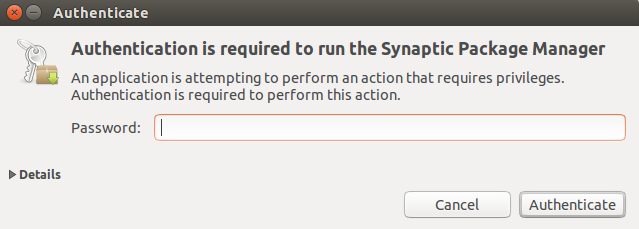
\includegraphics[scale=0.55]{password.png}
\caption{Enter the system password here}
\end{center}  
\end{figure}
\vspace{1cm}
\flushleft Once the Synaptic Package Manager is Opened, in the search box type OpenFOAM.

\begin{figure}[ht]  
\begin{center}  
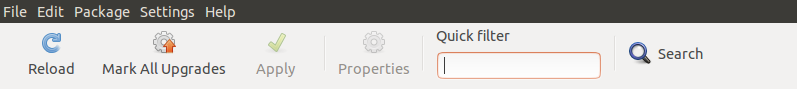
\includegraphics[scale=0.4]{searchbox.png}
\caption{Type OpenFOAM in the search box}
\label{searchbox}
\end{center}  
\end{figure}

\flushleft You will see both OpenFOAM-2.3.0 and Paraview-4.1.0. Right Click Both of them for installation and click Apply to install, Fig \ref{searchbox}. This will take a while for installation depending upon your internet speed.

\begin{figure}[ht]  
\begin{center}  
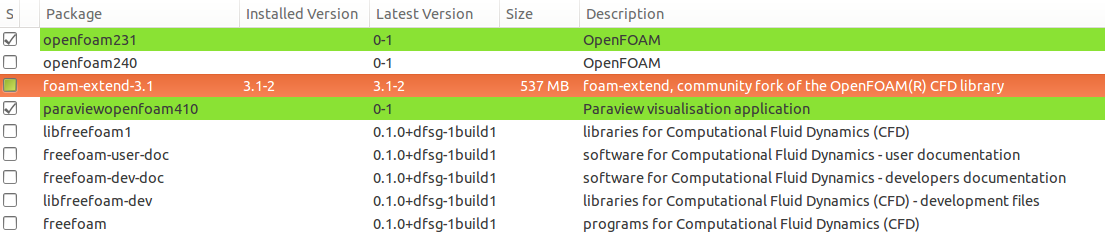
\includegraphics[scale=0.33]{mark.png}
\caption{Click on OpenFOAM and Paraview to Mark and Install}
\label{searchbox}
\end{center}  
\end{figure}

\flushleft OpenFOAM can also be downloaded and installed using the OpenFOAM website as follows. 
\begin{itemize}
\item On your browser type \textbf{www.openfoam.com/download} 
\item Go to Ubuntu Debian Installation
\item Under the first point of Installation copy the command line and paste this in your terminal window
\item Open the terminal window by pressing \textbf{Ctl+Alt+t} keys simultaneously on your keyboard or you can also open it using the search icon on top of the Launchbar

\begin{figure}[ht]  
\begin{center}  
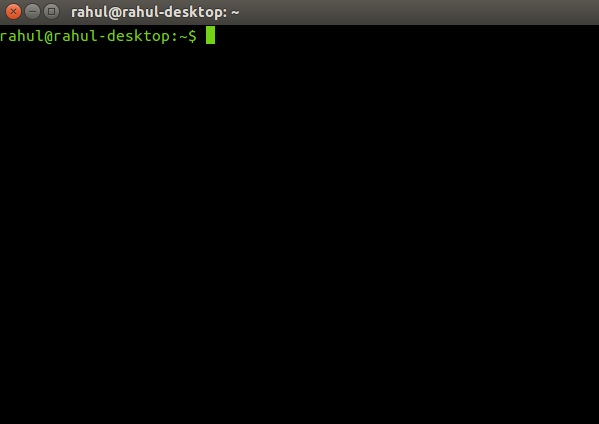
\includegraphics[scale=0.28]{terminal.png}
\caption{Press Ctrl+Alt+t keys to open up terminal window}
\label{terminal}
\end{center}  
\end{figure}

\item For complete installation for OpenFOAM and Paraview follow the steps under installation

\end{itemize}

\flushleft To configure the installed software we need to edit the bashrc file. To do this open a new command terminal and type \textbf{gedit $\sim$$\slash$.bashrc} and press enter

\begin{figure}[ht]  
\begin{center}  
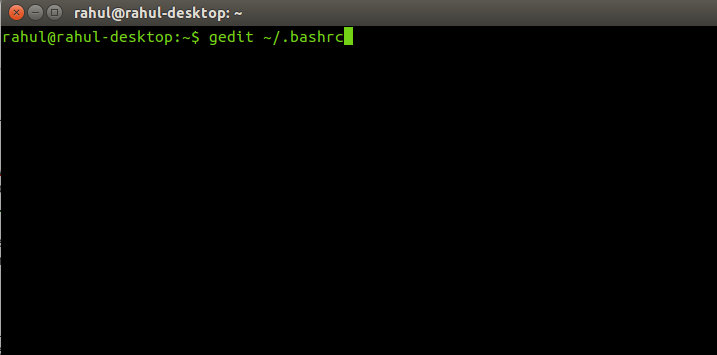
\includegraphics[scale=0.4]{bash.png}
\caption{Open the bashrc file}
\label{terminal}
\end{center}  
\end{figure}

\flushleft After the bashrc file is opened scroll down to the bottom of the file. Then go back to your browser (OpenFOAM download page) and scroll down to \textbf{User Configuration}.  

\flushleft Copy the second point \textbf{source /opt/openfoam230/etc/bashrc} under this heading and paste it at the bottom of the bashrc file. Save it and close the file.

\flushleft To check weather OpenFOAM is installed properly open a new command terminal and type \textbf{icoFoam -help} and press enter. You will see a "Usage" message on your terminal screen, Fig \ref{usage} which shows that the installation is done.

\begin{figure}[ht]  
\begin{center}  
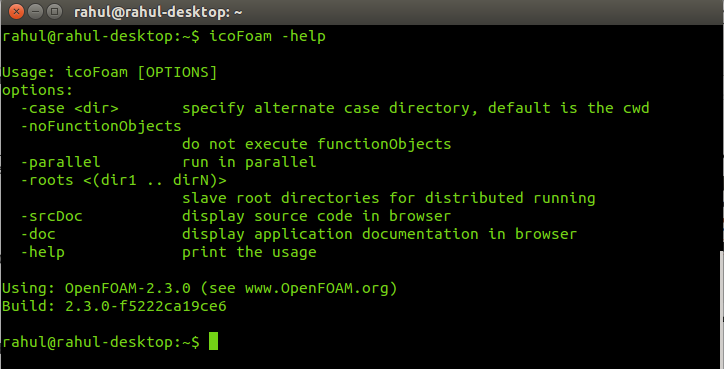
\includegraphics[scale=0.5]{usage.png}
\caption{Usage message appears which shows OpenFOAM is correctly installed}
\label{usage}
\end{center}  
\end{figure}

\flushleft Now we will set up the working directory and copy the tutorial folder. Follow the steps given below. 
\begin{enumerate}
\item Open up a new terminal and type \textbf{mkdir -p $\$$FOAM$\_$RUN} and press enter
\item Now type \textbf{cp -r $\$$FOAM$\_$TUTORIALS} \textbf{$\$$FOAM$\textunderscore$RUN} and press enter. This will copy the tutorials folder into the run directory.
\end{enumerate}


\flushleft Alternate way to install OpenFOAM and Paraview is by Compiling the Source code available under the header of \textbf{Source Pack} Installation on the OpenFOAM website. Download the tar files. Create a folder in your Home directory by the name OpenFOAM and paste the tar files in that folder. Extract the files in that folder.

\flushleft Follow the steps given on the OpenFOAM source pack installation page to complete the installation. Since we compile the source code it might take a few hours to complete.

\flushleft We will solve an example problem here by the name Lid Driven Cavity. It is a two dimensional problem where the upper plate moves and other three sides of the plate are fixed, \ref{lid}. The solver we use here is icoFoam which is an Transient solver for incompressible flow.

\begin{figure}[ht]  
\begin{center}  
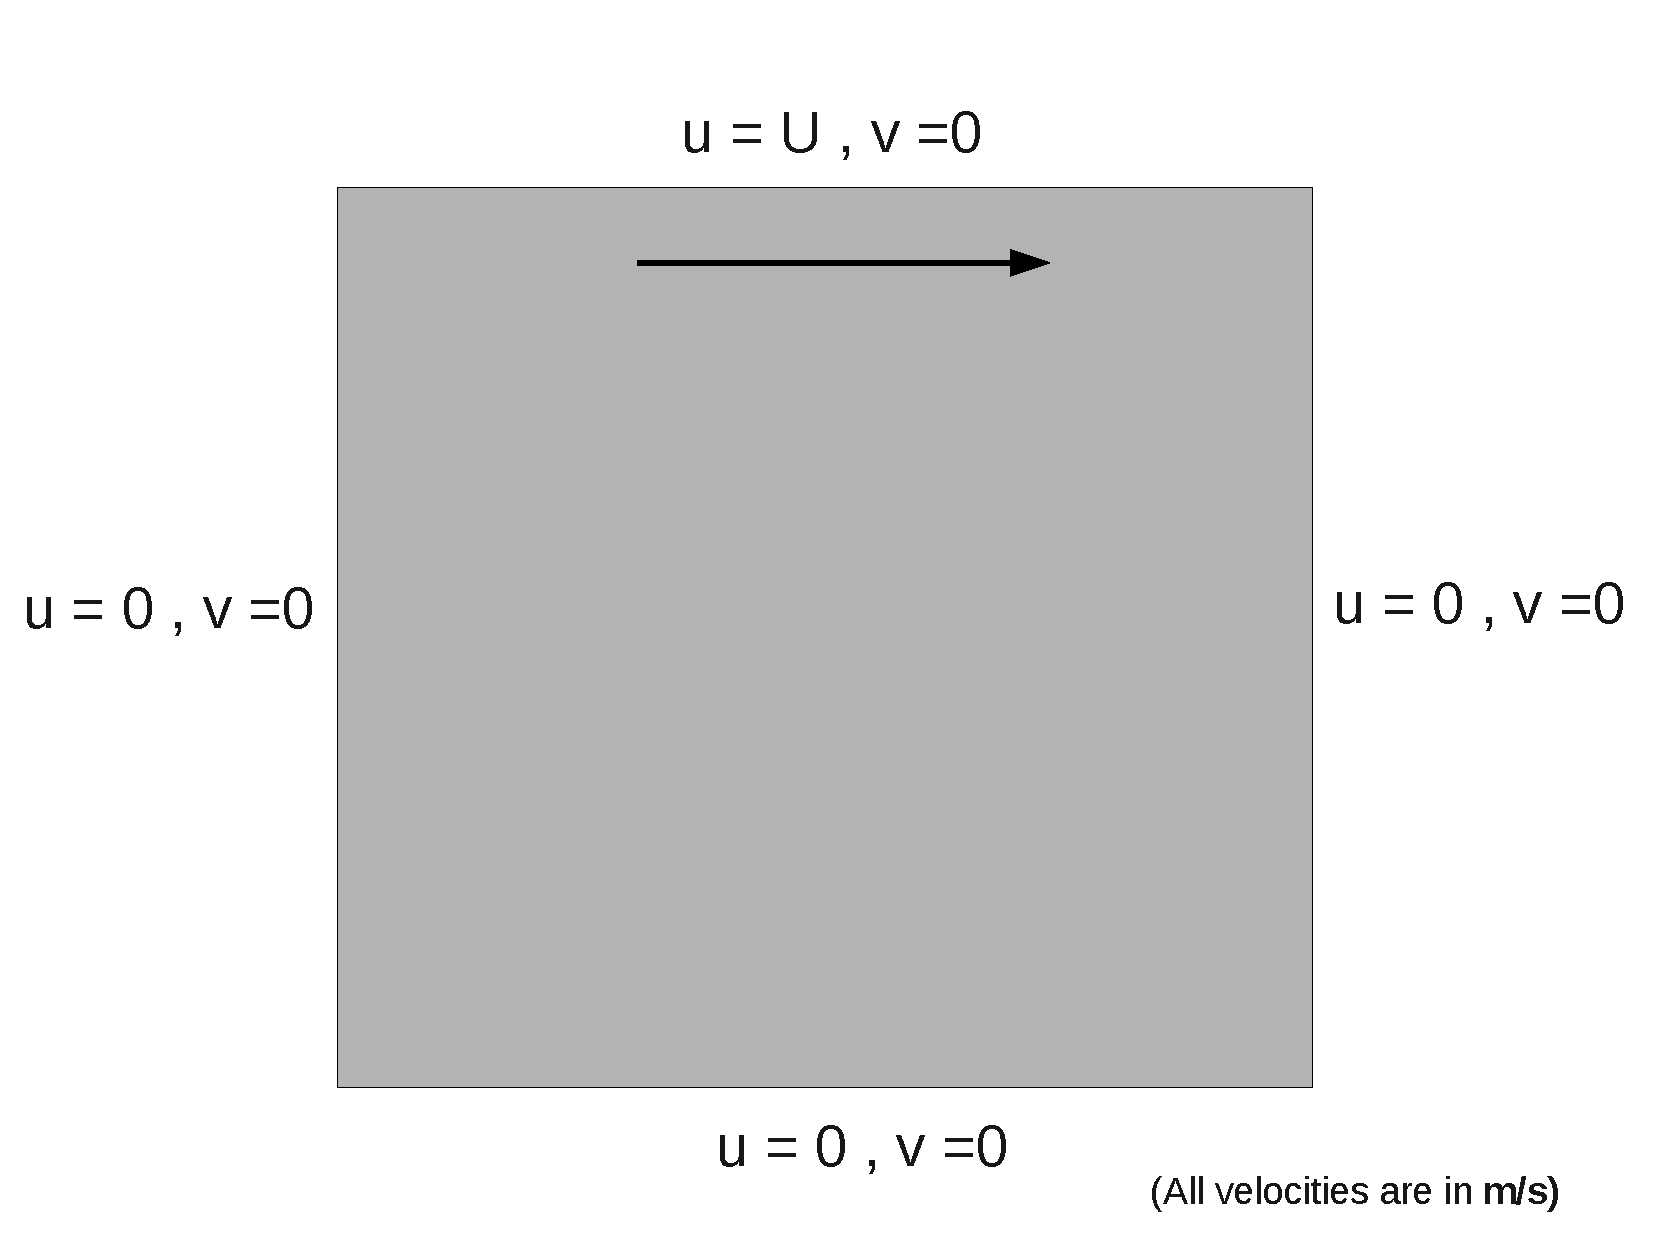
\includegraphics[scale=0.3]{liddrivencavity.pdf}
\caption{Example problem solved after OpenFOAM installation}
\label{lid}
\end{center}  
\end{figure}

\flushleft In the terminal copy paste the path given below :\\

\center cd OpenFOAM/OpenFOAM-2.3.0/run/tutorials/incompressible/icoFoam/cavity

\flushleft The geometry now needs to be meshed. This can be done using the blockMesh utility of OpenFOAM. In the command terminal type \textbf{blockMesh} and press enter which completes the meshing, Fig \ref{mesh}

\begin{figure}[ht]  
\begin{center}  
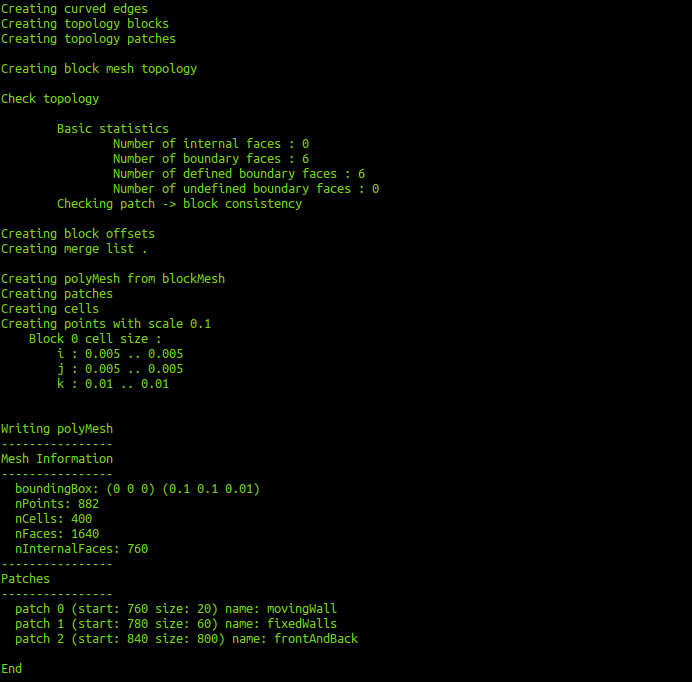
\includegraphics[scale=0.3]{blockMesh.png}
\caption{blockMesh utility for Meshing in OpenFOAM}
\label{mesh}
\end{center}  
\end{figure}
\vspace{1cm}
\flushleft Once meshing is done we now run the solver by typing \textbf{icoFoam} in the command terminal. The iteration running can be seen in the terminal window, Fig \ref{solver}. We have reached the solving point.

\begin{figure}[ht]  
\begin{center}  
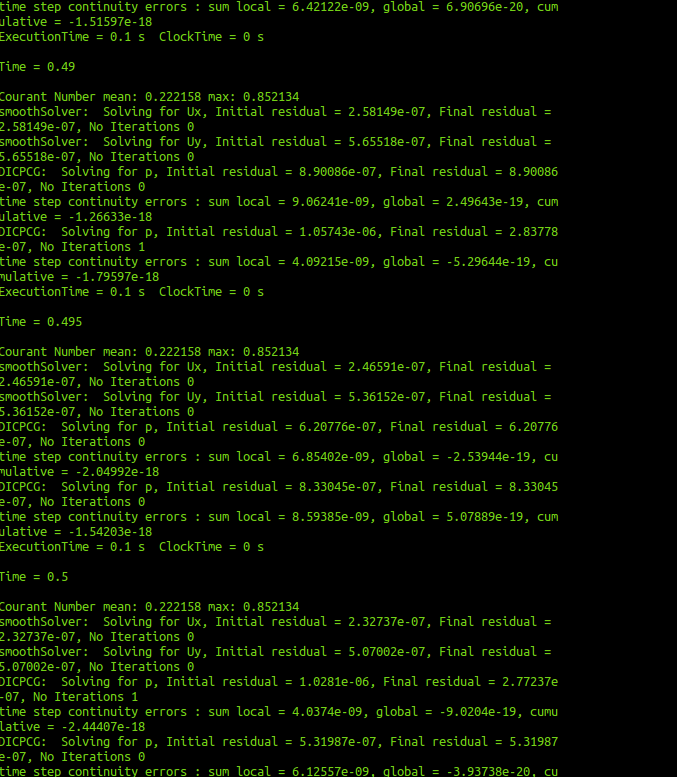
\includegraphics[scale=0.3]{solver.png}
\caption{Terminal shows the iterations running}
\label{solver}
\end{center}  
\end{figure}

\flushleft The results can be Visualized using Paraview. To open paraview in your terminal type \textbf{paraFoam} and press enter. This will open up the paraview window, Fig \ref{pv}.

\begin{figure}[ht]  
\begin{center}  
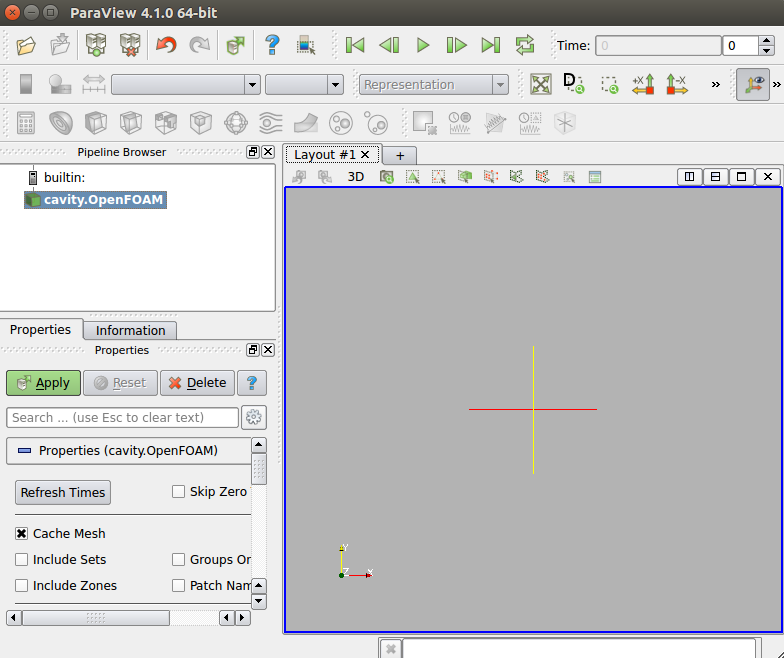
\includegraphics[scale=0.32]{paraview.png}
\caption{Paraview window}
\label{pv}
\end{center}  
\end{figure}

\vspace{0.8cm}
\flushleft Click on the Apply button on the left hand side of the \textbf{Object Inspector} Menu to view the Geometry, Fig\ref{geom}.

\begin{figure}[ht]  
\begin{center}  
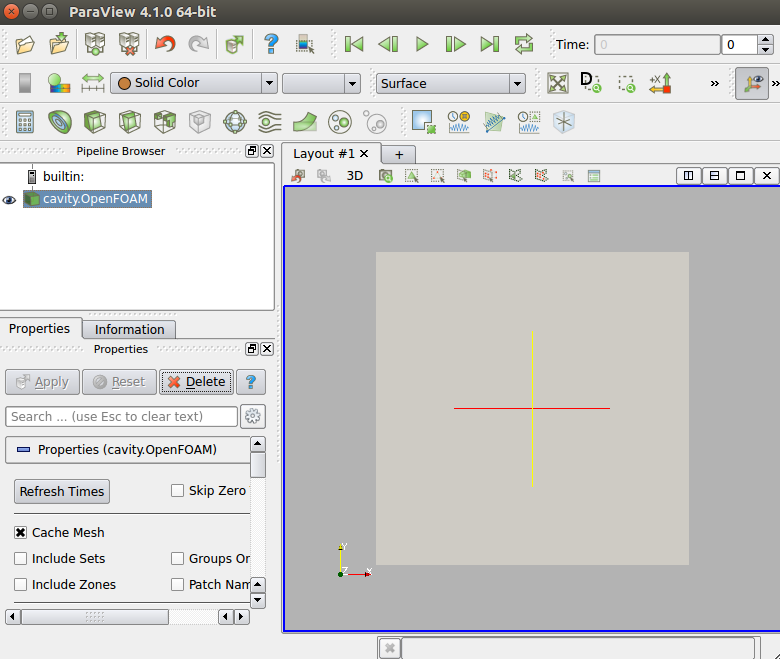
\includegraphics[scale=0.32]{geom.png}
\caption{Geometry seen in the Paraview Window}
\label{geom}
\end{center}  
\end{figure}

\flushleft To check the Boundary conditions scroll down the object inspector menu and go down to mesh parts and uncheck internal mesh option and click Apply. You can see that the geometry disappears, Fig \ref{parts}.

\begin{figure}[ht]  
\begin{center}  
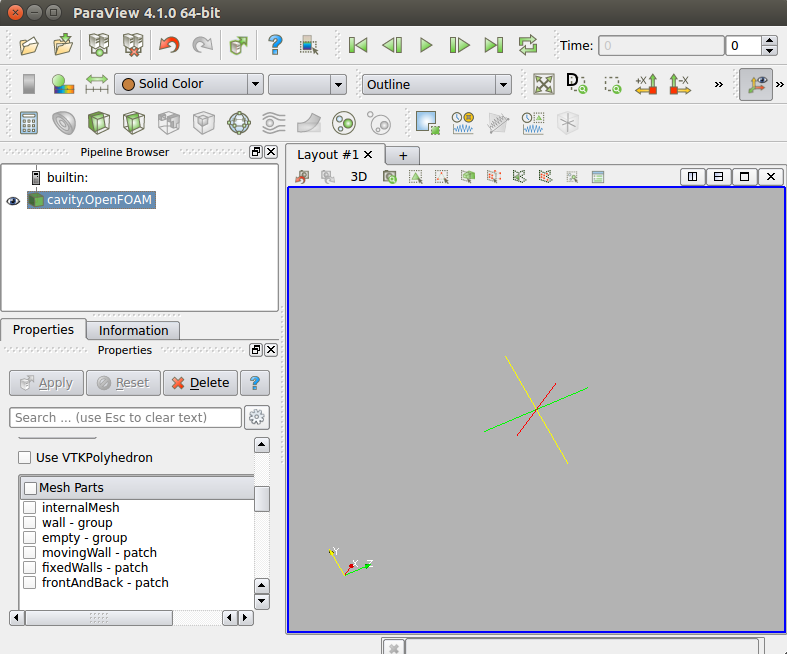
\includegraphics[scale=0.32]{part1.png}
\caption{Uncheck the internal mesh option}
\label{parts}
\end{center}  
\end{figure}

\vspace{1.5cm}
\flushleft Now click on the checkbox for movingWall and fixedWall and click the Apply button. You can see the moving wall and fixedWall in the paraview window, Fig \ref{part2}. Also uncheck the movingWall to see the fixedWalls in the paraview, Fig \ref{part3}.

\begin{figure}[ht]  
\begin{center}  
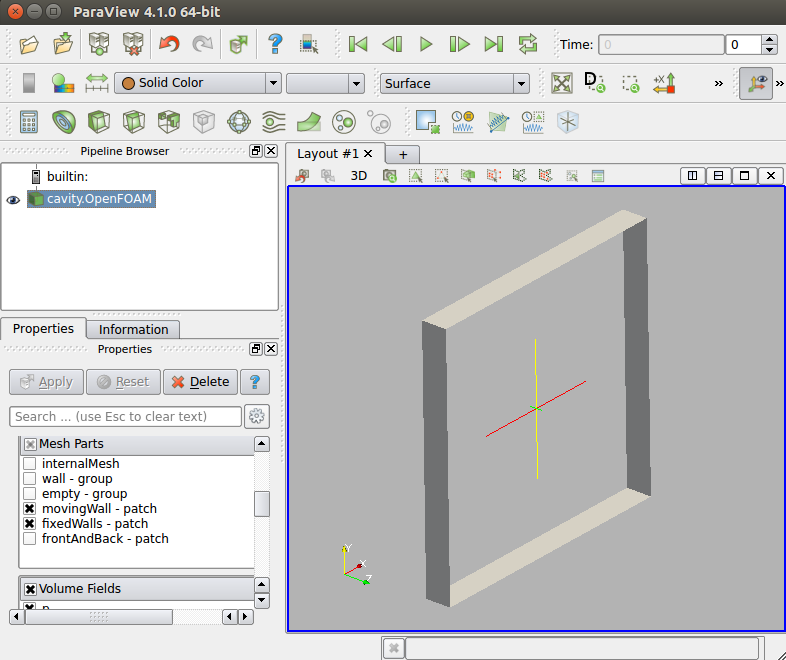
\includegraphics[scale=0.32]{part2.png}
\caption{Check for the moving and fixedWalls in paraview window}
\label{part2}
\end{center}  
\end{figure}

\begin{figure}[ht]  
\begin{center}  
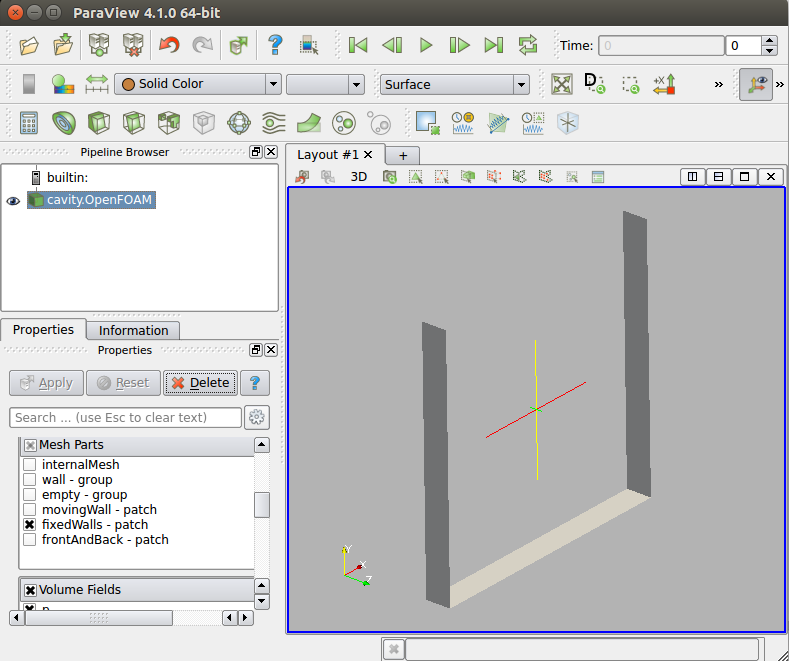
\includegraphics[scale=0.32]{part3.png}
\caption{FixedWalls appear in the paraview window}
\label{part3}
\end{center}  
\end{figure}



\end{document}
